\documentclass[11pt]{article}

\usepackage[a4paper,margin=2.6cm]{geometry}
\usepackage{fontspec}
\setmainfont{Malgun Gothic}[BoldFont={Malgun Gothic Bold}]
\usepackage{amsmath,amssymb}
\usepackage{graphicx}
\usepackage{booktabs}
\usepackage{xcolor}
\usepackage{hyperref}
\usepackage{caption}
\usepackage{kotex}

\hypersetup{colorlinks=true, linkcolor=blue!50!black, citecolor=blue!50!black, urlcolor=blue!40!black}

% ex13 dataset numbers (from analysis/ex13_check.json, D:/CAE_datasets_raw/deepjeb_ver_fea)
\newcommand{\NTRAIN}{1,697}
\newcommand{\NINFER}{424}
\newcommand{\PTRAIN}{209}
\newcommand{\PINFER}{54}
\newcommand{\NODESMIN}{4,995}
\newcommand{\NODESMAX}{5,007}
\newcommand{\UZRET}{0.9988}
\newcommand{\UZRETPONE}{0.9934}
\newcommand{\VMRET}{0.69}
\newcommand{\VMRETLO}{0.50}
\newcommand{\VMRETHI}{0.78}
\newcommand{\NBOLT}{127}
\newcommand{\NLUG}{93}
\newcommand{\SMUX}{0.064}
\newcommand{\SMUY}{0.087}
\newcommand{\SMUZ}{0.052}
\newcommand{\SMVM}{0.263}
\newcommand{\GSPLIT}{1,365/146/186개}
\newcommand{\VMNODAL}{0.95}
\newcommand{\VMSMALL}{0.74}

\title{\textbf{DeepJEB 수직하중 FEA 재해석\\
OpenRadioss tet4로 2,121개 브래킷을 다시 풀고, 논문 라벨과 비교하고,\\
MGN 학습용 데이터셋(ex13)으로 만들기}}
\author{AI-CAE4ALL}
\date{2026년 9월}

\begin{document}
\maketitle

\begin{abstract}
\noindent
DeepJEB(arXiv:2406.09047)는 제트엔진 브래킷 2,138개의 형상과 네 가지 하중
조건의 OptiStruct 해석 결과를 공개한 데이터셋이다. 하지만 결과는 형상당
스칼라 몇 개(최대 변위, 최대 응력)뿐이고, 절점 필드는 절점 순서가 사라져
형상과 짝지을 수 없다. 그래서 수직하중(35.6~kN, $+z$) 조건을 전부 우리가
다시 풀었다. 메쉬는 우리 tet4(표면 0.7~mm)로 만들었고, 솔버는 OpenRadioss
implicit linear static이다. 경계조건은 원본 해석 파일(.fem)을 쓰지 않고
\textbf{형상만 보고 정하는 기하 규칙}으로 잡았다. 볼트 구멍 4개의 벽은
고정(RBE2)하고, 러그 두 귀의 구멍 벽에는 RBE3로 하중을 건다. 이 규칙은
나중에 생성 모델이 만든 형상을 검증할 때도 그대로 쓴다.
2,138개 중 \textbf{2,121개(99.2\%)}를 풀었다. 나머지 17개는 모두 메쉬
단계에서 실패했고, 해석 단계의 실패는 없다. 최대 수직변위 $\max|u_z|$는
라벨 대비 비율 중앙값이 \textbf{0.988}(p05--p95 0.979--0.993), 평균 절대오차가
1.28\%, Spearman 상관이 \textbf{0.9999}다. 약 $-1.2\%$인 편향은 두 요인으로
분해된다. 하나는 기하 BC 규칙($-0.6\%$), 다른 하나는 tet4 강성($-0.8\%$)이다.
논문의 tet10 메쉬와 논문의 러그 절점을 그대로 쓰면 라벨을 0.08\% 이내로
재현한다. 최대 응력은 정의가 달라서(라벨은 tet10 절점 응력, 우리는 tet4 요소
평균) 직접 비교할 수 없다. 결과는 5,000절점 표면 그래프로 줄여서 MGN 형식
데이터셋 \texttt{ex13\_deepjeb\_ver}로 만들었다(학습 \NTRAIN{}개, 평가
\NINFER{}개). 분할은 SDFFlow ex1\_deepjeb의 부모 단위 분할을 그대로 따른다.
\end{abstract}

\tableofcontents

% =====================================================================
\section{해석 조건}
% =====================================================================

\begin{figure}[h]
  \centering
  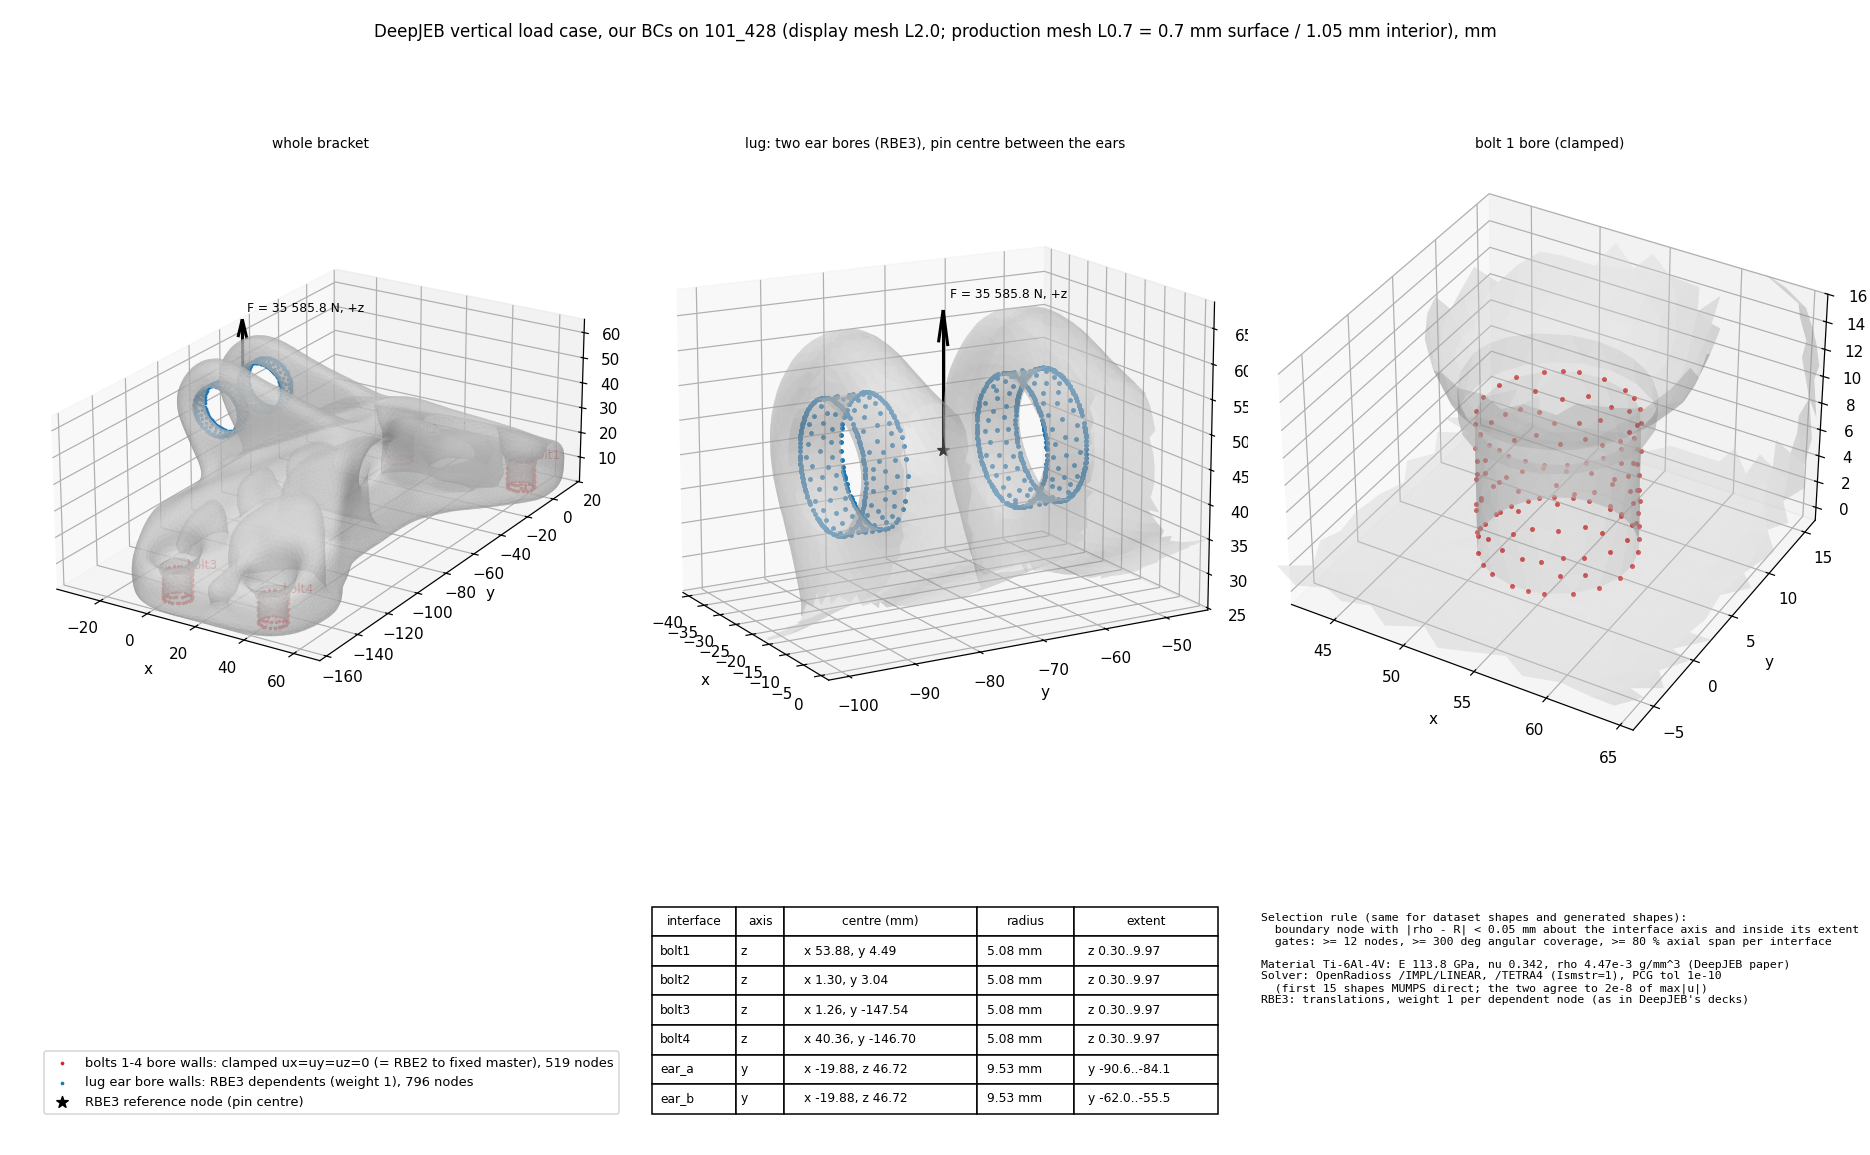
\includegraphics[width=\textwidth]{figures/fig1_bc_setup.png}
  \caption{수직하중 조건과 우리 경계조건(형상 101\_428). 빨강: 볼트 1--4 구멍 벽,
  세 방향 변위 고정(고정 master에 RBE2로 묶은 것과 같다). 파랑: 러그 두 귀의
  구멍 벽, RBE3 종속 절점. 별: RBE3 기준점(핀 중심, 두 귀 사이의 빈 공간).
  이 점에 $F=35\,585.8$~N을 $+z$로 건다. 그림은 보기 쉽게 L2.0 메쉬로
  그렸고, 실제 해석은 L0.7 메쉬로 했다. 아래 표는 모든 형상에 공통인 인터페이스
  치수다(DeepJEB의 FieldMesh 421개에서 측정).}
  \label{fig:bc}
\end{figure}

\begin{table}[h]
\centering\small
\begin{tabular}{@{}lll@{}}
\toprule
항목 & 논문 (DeepJEB 라벨) & 우리 \\
\midrule
솔버 & OptiStruct linear static & OpenRadioss \texttt{/IMPL/LINEAR} (PCG, tol $10^{-10}$) \\
요소 & 2차 사면체(tet10), 평균 약 2~mm & 1차 사면체(tet4), 표면 0.7~mm / 내부 1.05~mm \\
재료 & Ti-6Al-4V, $E=113.8$~GPa, $\nu=0.342$ & 동일 \\
하중 & 35.6~kN (8,000~lbf) $+z$, 러그에 RBE3 & 동일 \\
구속 & 볼트 4개 RBE2 고정 & 동일(구멍 벽 절점 3방향 고정) \\
BC 절점 선택 & 원본 .fem에 정의된 절점 & \textbf{형상에서 기하 규칙으로 선택} \\
\bottomrule
\end{tabular}
\caption{해석 조건. 다른 것은 요소 차수·크기와 BC 절점을 고르는 방법 두 가지뿐이다.}
\label{tab:setup}
\end{table}

DeepJEB의 모든 브래킷은 같은 인터페이스 형상을 불리언으로 붙여서 만들었다.
그래서 볼트 구멍과 러그 구멍의 위치와 반지름이 모든 형상에서 같다.
FieldMesh(DeepJEB가 공개한 OptiStruct tet10 메쉬) 421개에 원을 맞춰 보면,
볼트 구멍 반지름은 5.080--5.082~mm, 중심 편차는 0.008~mm 이하, 러그 구멍
반지름은 9.524--9.552~mm, 중심 편차는 0.025~mm 이하였다(그림~\ref{fig:bc} 아래 표). 이 상수만 있으면
형상 파일만으로 BC 절점을 고를 수 있다.

% =====================================================================
\section{방법}
% =====================================================================

\subsection{형상과 메쉬}

입력은 DeepJEB가 공개한 \texttt{SurfaceMesh/<item>.stl}(Inspire CAD의
삼각형화 결과)이다. 형상마다 다음 순서로 tet4 메쉬를 만든다.
\begin{enumerate}
\item \textbf{불러오기.} 1e-4~mm 안의 중복 절점을 합치고 가장 큰 덩어리만 남긴다.
      STL에는 부피가 0인 중복 껍질이 붙어 있다.
\item \textbf{재메쉬.} pymeshlab 등방 재메쉬(Botsch--Kobbelt)로 모서리 길이를
      0.7~mm에 맞춘다. 30° 넘는 특징선은 보존하고, 표면 편차는 0.035~mm 이하로 묶는다.
\item \textbf{정리.} 특징선 두 개가 작은 각으로 만나는 곳에 남는 바늘·뚜껑
      모양 삼각형(형상당 약 100개)을 edge collapse와 edge flip으로 고친다.
      접힌 삼각형 쌍(이면각 0)도 제거한다. 이게 남으면 Delaunay가 경계를 거부한다.
\item \textbf{사면체.} gmsh로 재매개화 없이 표면 분류만 하고, 정리한 삼각형을 그대로
      경계로 쓴다. 내부는 HXT Delaunay와 Netgen 최적화로 채우고, 내부 크기는
      1.05~mm 이하로 둔다. 실패하면 표면 길이를 $\times0.97$, $\times1.03$으로 바꿔
      다시 시도한다.
\item \textbf{게이트.} 부피가 라벨 CSV 부피와 맞는지, 원래 STL과의 Hausdorff
      거리, 최소 SICN(sliver 검사)을 확인한다.
\end{enumerate}
최종 메쉬는 형상당 중앙값 50만 절점, 280만 요소다(범위 24만--98만 절점).
부피는 라벨 대비 0.9996(평균 오차 0.04\%)이다.

\subsection{경계조건 규칙}

메쉬 경계 절점 중 인터페이스 축으로부터의 거리 $\rho$가 구멍 반지름과
0.05~mm 안에서 같고 벽의 축방향 범위 안에 있는 절점을 고른다.
\begin{itemize}
\item \textbf{볼트 $k$ (RBE2, 고정).} $|\rho-5.08|<0.05$, $z\in[0.30, 9.97]$.
      고정 master에 RBE2로 묶는 것은 종속 절점을 3방향 모두 고정하는 것과
      정확히 같으므로 \texttt{/BCS 111}로 건다.
\item \textbf{러그 (RBE3).} $y$축 기준 $|\rho-9.53|<0.05$이고 두 귀의 $y$ 범위
      $[-90.6,-84.1]$, $[-62.0,-55.5]$ 안에 있는 절점을 고른다. 이 절점들을
      기준점 $(-19.88,\,-73.05,\,46.72)$의 RBE3 종속 절점(가중치 1, 병진만)으로
      두고 기준점에 $F_z=35\,585.8$~N을 건다.
\item \textbf{게이트.} 구멍마다 절점 12개 이상, 원주 커버리지 300° 이상, 벽 높이의
      80\% 이상을 덮어야 한다. 못 채우면 그 형상은 BC 오류로 처리한다.
\end{itemize}
L0.7 메쉬에서 고정 절점은 형상당 중앙값 3,019개, 러그 절점은 2,349개였다.
이 규칙은 원본 .fem을 보지 않는다. 그래서 생성 모델이 만든 새 형상에도 똑같이
쓸 수 있고, 이것이 이 방식을 택한 이유다.

\subsection{솔버와 솔버 검증}

OpenRadioss(Mg-mm-s 단위계)로 \texttt{/IMPL/LINEAR} 한 스텝을 푼다.
요소는 \texttt{/TETRA4}(1점 적분, \texttt{Ismstr=1} 소변형)이다. 다음을 확인했다.
\begin{itemize}
\item \textbf{요소 정식화.} 외팔보 검증에서 \texttt{Itetra10=2}(tet10을 tet4 시간간격으로
      쓰는 변형)는 implicit linear에서 10--40\% 너무 유연했다. 그래서 tet10 비교에는
      \texttt{Itetra10=1000}(4점 적분)을 썼다. \texttt{Ismstr} 기본값(대변형)은
      변위는 같지만 자유 절점에 최대 9~N의 잔류 반력을 남긴다. \texttt{Ismstr=1}을
      쓰면 볼트 반력의 합이 $-F$와 $10^{-7}$ 이내로 맞는다.
\item \textbf{평형.} 모든 형상에서 볼트 반력의 합을 $-F$와 비교했다. 상대오차 중앙값은
      $1.4\times10^{-7}$, 최대 $5.6\times10^{-7}$이다.
\item \textbf{PCG 대 MUMPS.} 처음 15개는 MUMPS 직접법으로 풀었다. L0.7에서 해석 하나가
      37--93~GB를 써서 공용 서버 메모리가 부족해졌고, 그 뒤로는 PCG(tol $10^{-10}$,
      3--5~GB)로 바꿨다. 같은 메쉬(102\_240, 55만 절점)에서 두 해법의 변위 차이는
      상대 $L_2$ $1.1\times10^{-10}$, 최대 변위 기준 $2\times10^{-8}$이었다.
\item \textbf{절점 매핑.} 결과를 NODE\_ID로 우리 절점 번호에 되돌린다. 좌표 최근접
      매칭은 변형된 위치 때문에 틀릴 수 있어서 쓰지 않는다. 매핑 안 된 절점과
      요소는 모든 형상에서 0개였다.
\end{itemize}

\subsection{메쉬 수렴}

5개 형상을 L = 2.0, 1.4, 1.0, 0.7~mm로 풀고, 같은 형상의 tet10 해(같은 BC 규칙)와
비교했다(표~\ref{tab:conv}). L0.7에서 tet4/tet10 비율은 0.985--0.996, 중앙값
0.992다. 그래서 L0.7을 채택했다. 더 줄이면 절점 수가 약 2.7배 늘어나고,
공용 서버에서 2,138개를 풀 수 없다.

\begin{table}[h]
\centering\small
\begin{tabular}{@{}lrrrr@{}}
\toprule
형상 & L 2.0 & L 1.4 & L 1.0 & L 0.7 \\
\midrule
101\_428 & 0.936 & 0.961 & 0.976 & 0.990 \\
195\_440 & 0.946 & 0.973 & 0.987 & 0.996 \\
377\_14  & 0.947 & 0.973 & 0.985 & 0.995 \\
533\_535 & 0.948 & 0.970 & 0.985 & 0.992 \\
77\_546  & 0.911 & 0.949 & 0.971 & 0.985 \\
\midrule
절점 수(중앙값) & 3.1만 & 7.5만 & 18.7만 & 51.4만 \\
\bottomrule
\end{tabular}
\caption{$\max|u_z|$의 tet4/tet10 비율. tet4는 강성이 약간 과대하게 나오는 요소라 1보다 작은
쪽에서 1로 수렴한다.}
\label{tab:conv}
\end{table}

\subsection{계산 규모}

aarl(공용 서버)에서 형상 하나씩 병렬 레인으로 풀었다. 형상당 해석 시간 중앙값은
12분, 메쉬를 포함하면 17분이다. 첫 실행에서 74개가 실패했다(메모리 감시로 중단 43,
엔진 오류 2, 메쉬 29). 같은 설정으로 다시 돌려 57개를 회복했고, 남은 17개는 모두
메쉬 단계의 실패다(\S\ref{sec:excluded}).

% =====================================================================
\section{결과: 라벨과의 비교}
% =====================================================================

\subsection{변위}

\begin{figure}[h]
  \centering
  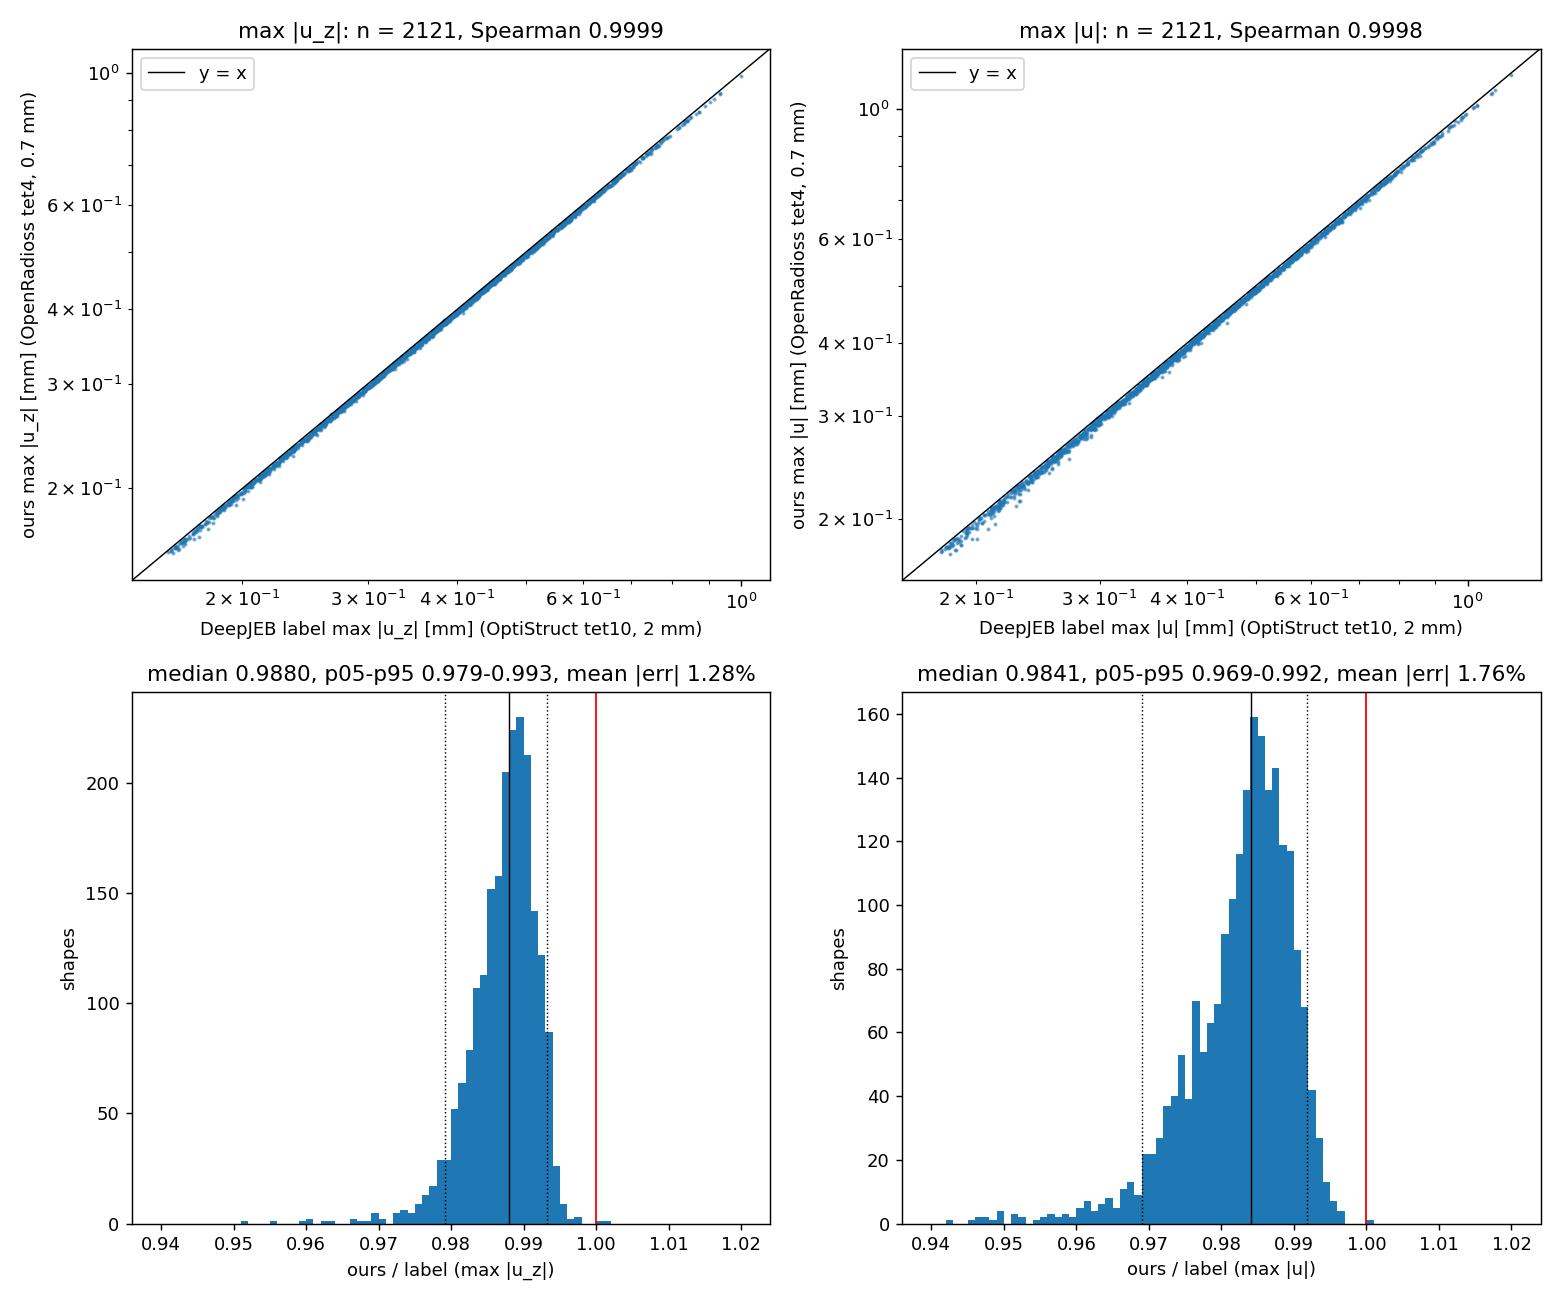
\includegraphics[width=0.92\textwidth]{figures/fig2_displacement_vs_labels.png}
  \caption{2,121개 형상의 최대 변위: 우리 해(OpenRadioss tet4 L0.7) 대 DeepJEB 라벨
  (OptiStruct tet10). 위: parity(로그 축). 아래: 비율 분포. 실선은 중앙값, 점선은 p05/p95,
  빨강은 1이다.}
  \label{fig:disp}
\end{figure}

\begin{table}[h]
\centering\small
\begin{tabular}{@{}lccccc@{}}
\toprule
지표 ($n=2121$) & 비율 중앙값 & p05--p95 & p25--p75 & 평균 $|$오차$|$ & Spearman \\
\midrule
$\max|u_z|$ & 0.988 & 0.979--0.993 & 0.985--0.990 & 1.28\% & 0.9999 \\
$\max|u|$   & 0.984 & 0.969--0.992 & 0.979--0.988 & 1.76\% & 0.9998 \\
부피        & 0.9996 & 0.9992--0.9999 & & 0.04\% & 1.0000 \\
\bottomrule
\end{tabular}
\caption{라벨 대비 비율(우리/라벨).}
\label{tab:disp}
\end{table}

순위는 사실상 완벽하게 보존된다(Spearman 0.9999). 최적화에서 "어느 형상이 더
좋은가"를 가리는 데 필요한 것은 이 순위다. 절대값은 약 1.2\% 작게 나오는데,
항상 작은 쪽이고 흩어짐도 좁다(p05--p95 폭 1.4\%). 가장 크게 벗어난 형상은
411\_488(0.952), 233\_537(0.956), 142\_538(0.959)이다.

\subsection{$-1.2\%$ 편향의 분해}

\begin{figure}[h]
  \centering
  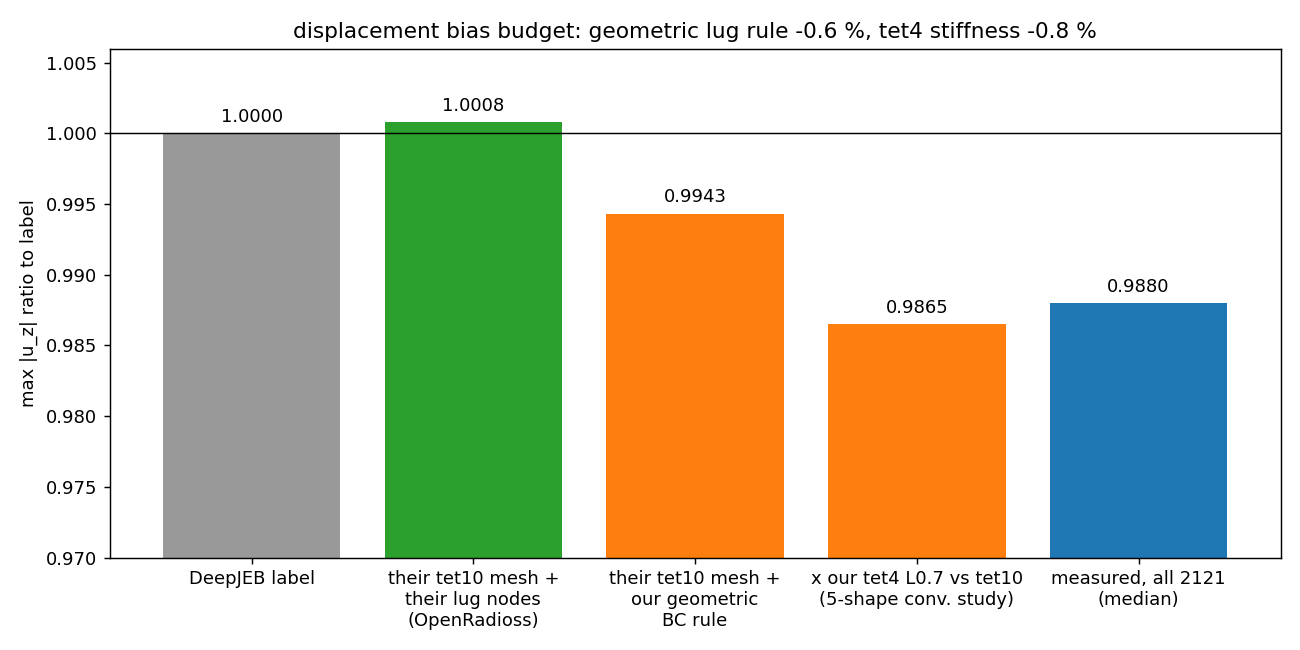
\includegraphics[width=0.78\textwidth]{figures/fig4_bias_budget.png}
  \caption{변위 편향 분해. 논문 메쉬와 논문 러그 절점을 쓰면 라벨을 재현하고(1.0008),
  러그 절점을 기하 규칙으로 바꾸면 0.9943, 여기에 tet4/tet10 비율(0.992)을 곱하면
  0.9865가 된다. 실측 중앙값은 0.988이다.}
  \label{fig:budget}
\end{figure}

FieldMesh가 있는 20개 형상으로 단계별로 확인했다(표~\ref{tab:v1}).
\begin{enumerate}
\item \textbf{체인 자체는 정확하다.} 논문의 tet10 메쉬와 .fem의 러그 절점을 그대로
      OpenRadioss에 넣으면 라벨과 0.08\% 차이다. 우리 deck 작성, RBE2/RBE3, 재료,
      단위는 모두 맞다.
\item \textbf{기하 BC 규칙: $-0.6\%$.} 같은 tet10 메쉬에서 러그 절점만 기하 규칙으로 바꾸면
      비율이 0.994가 된다. 20개 모두에서 우리 러그 절점은 .fem의 RBE3 절점의 부분집합이다
      (101\_428: 우리 777개, .fem 817개, 공통 777개). .fem에만 있는 15--53개는 거의 모두
      귀 구멍의 축 방향 가장자리($y\approx-55.5,\,-62,\,-84,\,-90.6$)에 있는 모서리 절점으로,
      우리 $y$ 구간 바로 밖이거나 반경 허용오차($\pm0.05$~mm) 밖에 있다.
      하중이 조금 더 넓은 벽에 퍼지므로 러그가 약간 더 부드럽게 반응한다.
\item \textbf{tet4 강성: $-0.8\%$.} 표~\ref{tab:conv}의 L0.7 tet4/tet10 중앙값은 0.992다.
\end{enumerate}
두 요인을 곱하면 $0.9943\times0.9921=0.9865$이고, 2,121개의 실측 중앙값 0.988과
0.15\% 차이다. 편향이 두 요인으로 설명된다.

\begin{table}[h]
\centering\small
\begin{tabular}{@{}lcccc@{}}
\toprule
20개 형상, 논문 tet10 메쉬 & $u_z$ 비율 중앙값 & 범위 & 평균 $|$오차$|$ & Spearman \\
\midrule
논문 러그 절점 & 1.0008 & 0.9999--1.0026 & 0.08\% & 1.000 \\
기하 BC 규칙 & 0.9943 & 0.9805--1.0061 & 0.70\% & 0.997 \\
\bottomrule
\end{tabular}
\caption{같은 메쉬에서 BC 절점 선택만 바꾼 비교.}
\label{tab:v1}
\end{table}

\subsection{응력}

\begin{figure}[h]
  \centering
  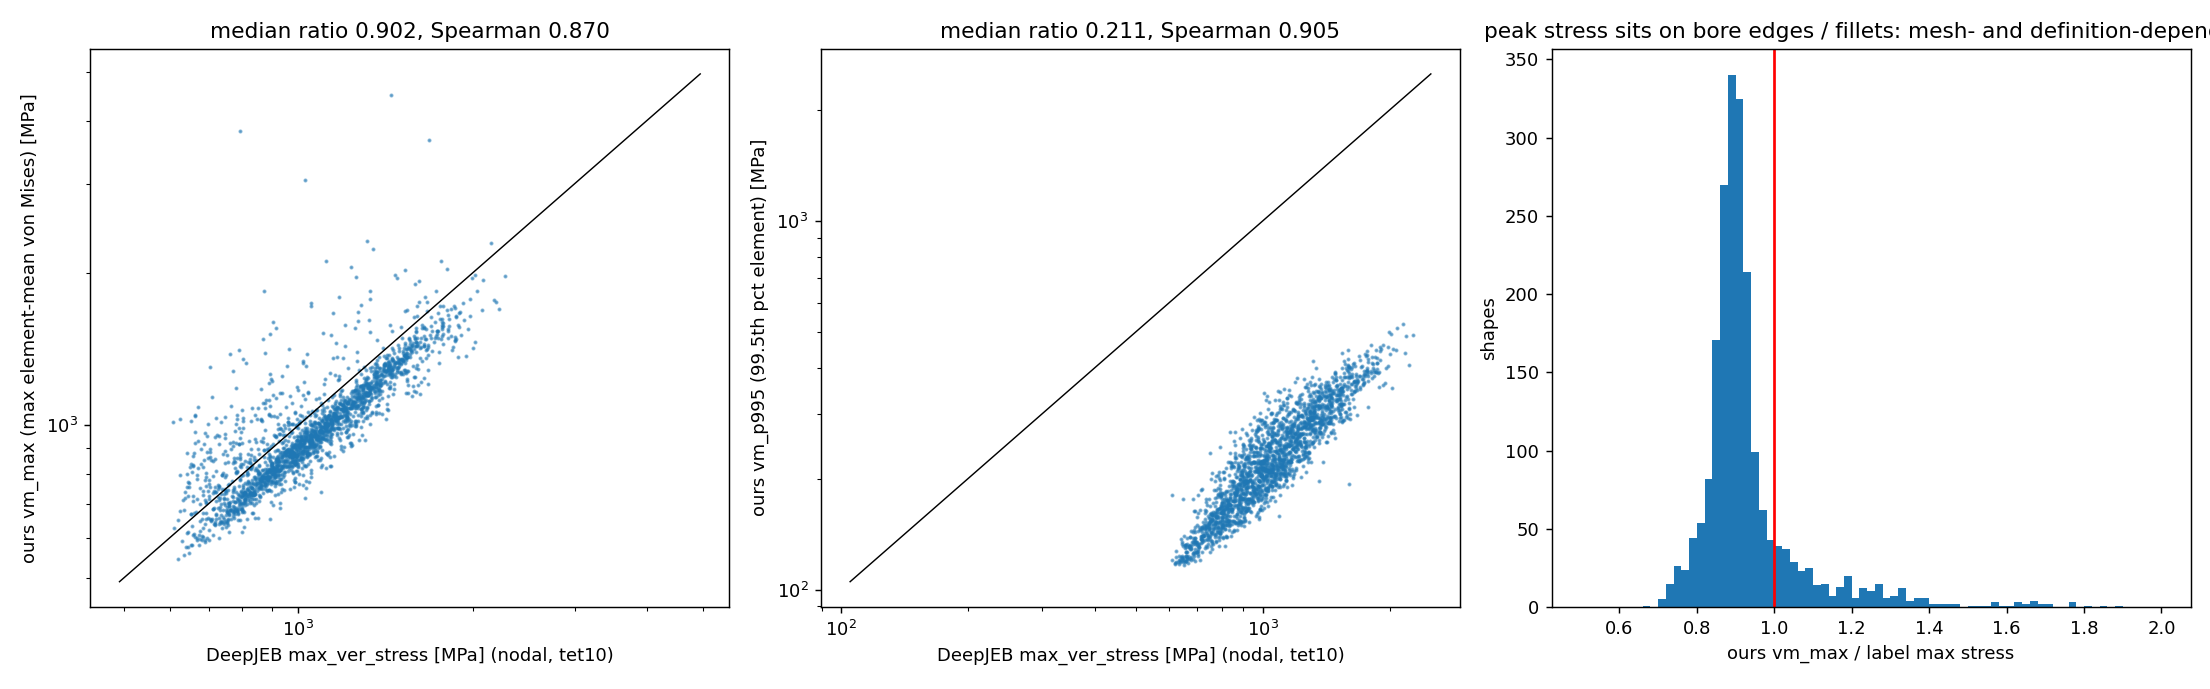
\includegraphics[width=\textwidth]{figures/fig3_stress_vs_labels.png}
  \caption{최대 von Mises 응력. 정의가 달라서(라벨은 tet10 절점 응력, 우리는 tet4 요소
  평균) 참고용으로만 보여 준다.}
  \label{fig:stress}
\end{figure}

vm\_max 비율 중앙값은 0.90, Spearman은 0.87이다. 흩어짐이 크고, 1.2--1.8배 쪽으로
꼬리가 있다. 원인은 두 가지다.
\begin{itemize}
\item \textbf{정의 차이.} 라벨은 tet10 절점 응력이다. 같은 tet10 메쉬에서 요소 평균을 계산하면
      라벨의 0.70배밖에 나오지 않는다(20개 형상, 0.65--0.88). 요소 평균은 구멍 가장자리의
      집중을 평균으로 깎는다.
\item \textbf{특이점.} 최대 응력은 볼트 구멍 가장자리나 필렛의 한 점에서 나오고, 메쉬에 따라
      바뀐다. 표~\ref{tab:conv}의 수렴 연구는 변위만 기록했으므로, 응력의 메쉬 수렴은
      이 보고서에서 확인하지 않았다.
\end{itemize}
그래서 검증 기준은 변위로 삼았다. 응력 최대값은 데이터셋에 기록만 하고 판정에는 쓰지 않는다.

% =====================================================================
\section{논문 결과와의 비교}
% =====================================================================

DeepJEB 논문은 FEA 결과의 분포 통계를 보고하지 않는다. 비교할 수 있는 수치는
Table~4의 surrogate 성능(최대 수직변위 예측)뿐이다: $R^2$ 0.9858--0.9901,
MAE $1.21$--$1.23\times10^{-2}$~mm, \textbf{MAPE 2.0--3.2\%}.

우리 재해석과 라벨의 차이(평균 1.28\%)는 논문의 가장 좋은 surrogate 오차(2.0\%)보다
작다. 그러므로 우리 결과를 학습 정답으로 써도 논문 수준의 surrogate 평가를 흔들지
않는다. 두 오차는 성격도 다르다. 우리 쪽은 거의 일정한 $-1.2\%$ 편향이고,
흩어짐(p05--p95 폭)은 1.4\%다. 이 평균 이동을 보정하면 남는 차이는 더 작다.
surrogate의 오차는 형상마다 방향이 바뀌는 오차다.

% =====================================================================
\section{제외된 17개}\label{sec:excluded}
% =====================================================================

\begin{table}[h]
\centering\small
\begin{tabular}{@{}lcp{7.2cm}@{}}
\toprule
원인 & 개수 & 형상 \\
\midrule
재메쉬 후 표면 자기교차 (PLC error) & 7 & 142\_284, 22\_552, 395\_62, 428\_437, 432\_235, 447\_331, 76\_411 \\
Delaunay가 요소 0개 생성 & 4 & 220\_623, 234\_488, 572\_547, 611\_428 \\
정리 후에도 표면이 닫히지 않음 & 3 & 16\_570, 208\_102, 559\_245 \\
세 크기 모두에서 sliver 요소 (SICN$<10^{-3}$) & 3 & 173\_152, 267\_80, 519\_447 \\
\bottomrule
\end{tabular}
\caption{제외된 형상. 모두 메쉬 단계의 실패이며, 해석 단계에서 실패한 형상은 없다.}
\end{table}

각 형상은 한 실행 안에서 표면 요소 길이 세 가지(0.679, 0.700, 0.721~mm)를 차례로
시도하고, 전체를 두 번 실행했다. 17개는 여섯 번의 시도 모두 실패했다. 첫 실행의 실패
기록 74개는 버리지 않고 \texttt{prod/\_failed\_pass1/}에 보관했다. 재메쉬 표면이
닫히지 않거나 자기교차하는 것으로 보아 원본 STL 쪽의 문제일 가능성이 있지만, STL을
직접 검사하지는 않았다.

% =====================================================================
\section{MGN 데이터셋 ex13\_deepjeb\_ver}
% =====================================================================

\begin{figure}[h]
  \centering
  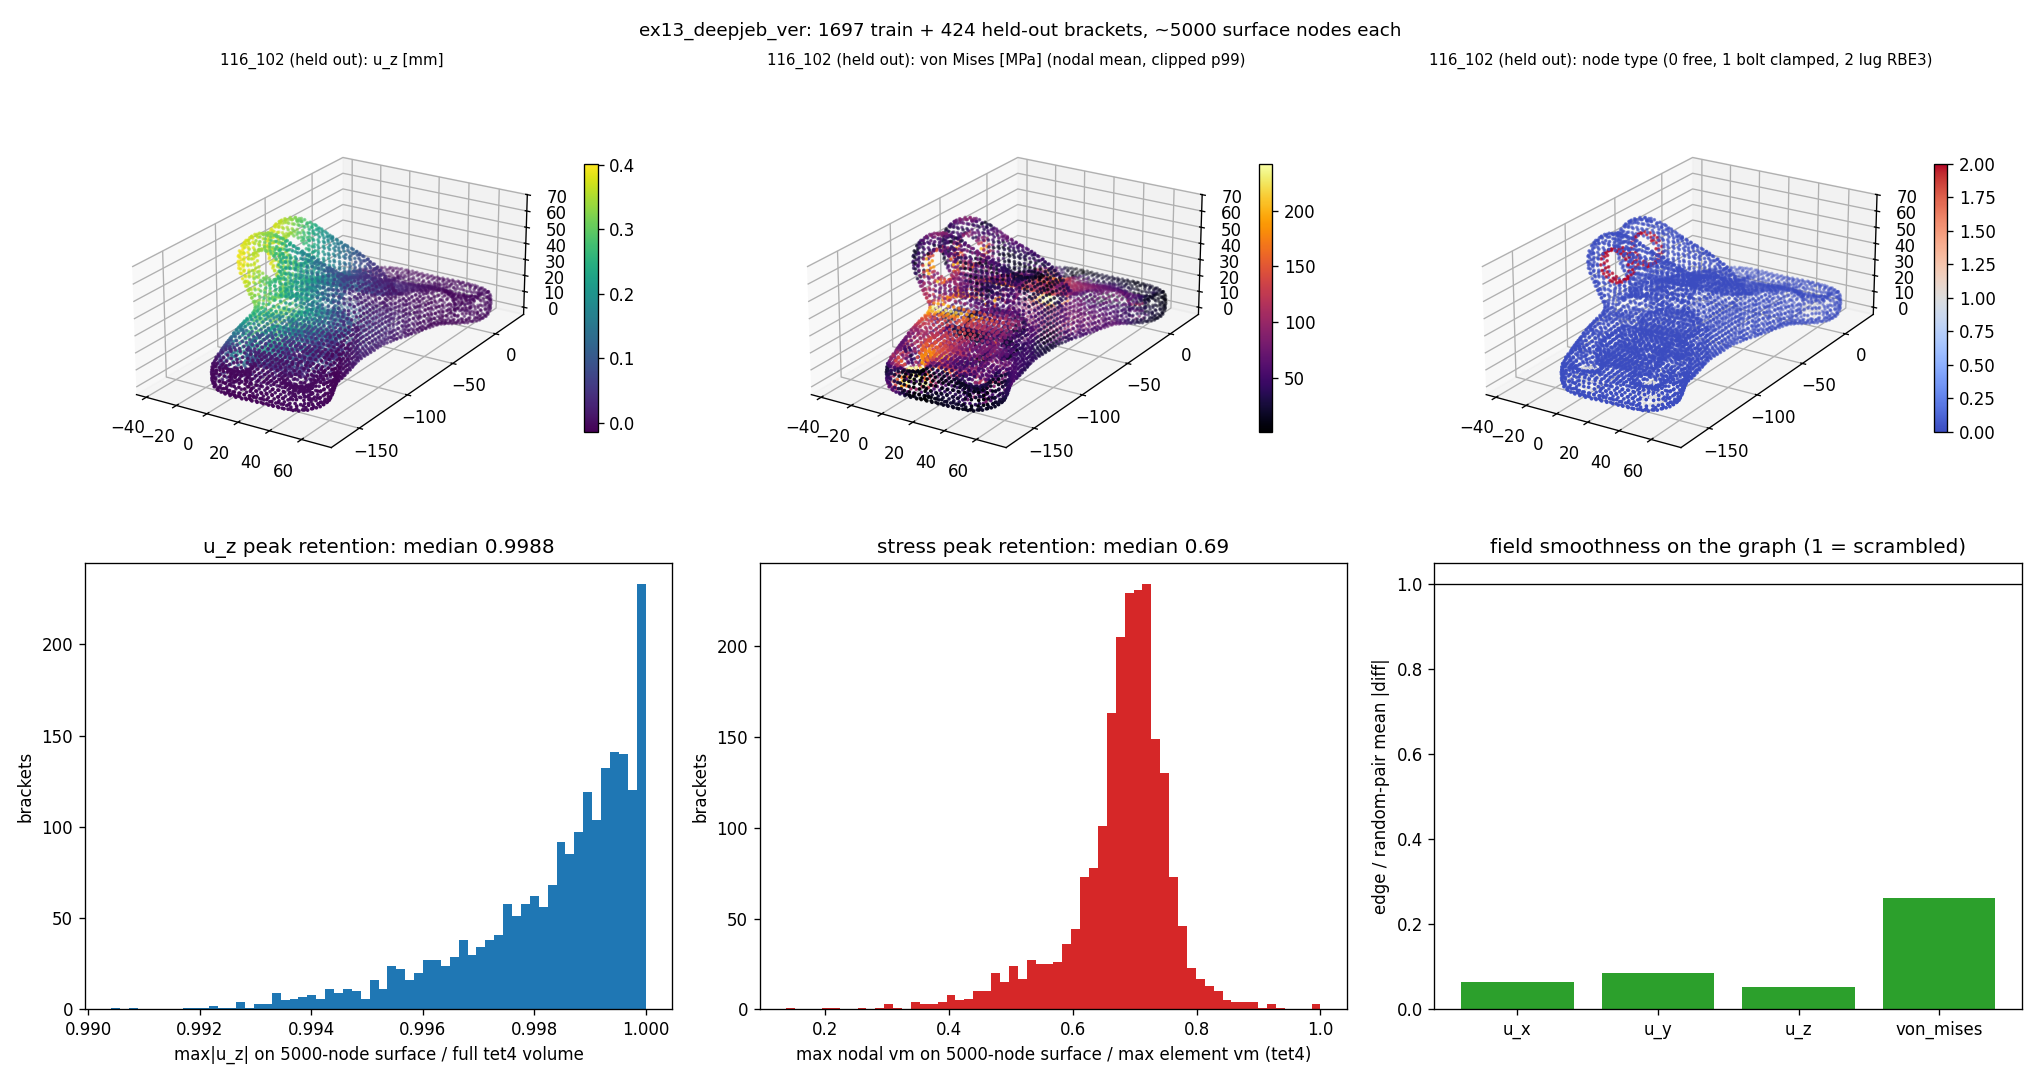
\includegraphics[width=\textwidth]{figures/fig5_ex13_dataset.png}
  \caption{ex13 데이터셋. 위: 평가 세트의 한 브래킷의 $u_z$, von Mises(절점 평균), 절점 유형.
  아래 왼쪽·가운데: 5,000절점 표면으로 줄인 뒤 최대값이 얼마나 남는지.
  아래 오른쪽: 그래프 위 필드의 매끄러움. 엣지로 이웃한 절점 차이를 무작위 절점 쌍의
  차이로 나눈 값이며, 필드가 뒤섞였으면 1이 된다.}
  \label{fig:ex13}
\end{figure}

\subsection{구성}

공유 메쉬 HDF5 규약(\texttt{data/\{id\}/\{nodal\_data, mesh\_edge, metadata\}})을 따른다.
\begin{itemize}
\item \textbf{행 8개.} \texttt{x, y, z}(mm) $|$ \texttt{u\_x, u\_y, u\_z}(mm),
      \texttt{von\_mises}(MPa) $|$ \texttt{node\_type}. 즉 \texttt{input\_var = output\_var = 4},
      \texttt{cond\_var 0}, 정적(T=1)이다. 절점 유형은 마지막 행에 둔다: 0 자유,
      1 볼트 구멍 벽(고정), 2 러그 구멍 벽(RBE3 하중).
      행이 8개라서 절점 유형을 \texttt{num\_features > 7}로 판단하는 모든 방법이 이 행을 읽는다.
\item \textbf{표면 그래프.} tet4 부피 메쉬의 경계면을 뽑고, von Mises를 절점으로 옮긴다
      (주변 요소의 단순 평균). 그다음 측지 정점 군집화로 약 5,000절점까지 줄인다
      (\NODESMIN--\NODESMAX 절점). 남는 절점은 모두 원래 해석 절점이다. 그래서 $u$, 응력,
      절점 유형은 보간값이 아니라 정확한 표본이다.
\item \textbf{분할.} SDFFlow의 \texttt{ex1\_deepjeb}(부모 단위 분할, seed 42)을 그대로 따른다.
      ex1 학습 형상은 \texttt{ex13\_deepjeb\_ver.h5}(\NTRAIN{}개, 부모 \PTRAIN{}개),
      ex1 평가 형상은 \texttt{ex13\_deepjeb\_ver\_infer.h5}(\NINFER{}개, 부모 \PINFER{}개)로 간다.
      DeepJEB 형상은 263개 부모에서 파생되고, 형제 형상은 거의 같은 모양이다. 그래서
      표본마다 \texttt{parent} 속성을 기록하고, config는 \texttt{split\_group\_attr parent}로
      학습 파일 안의 train/val/test도 부모 단위로 나눈다.
\item \textbf{메타데이터.} 표본마다 부피 메쉬 기준 $\max|u_z|$, $\max|u|$, 요소 vm\_max/p99.5,
      부피, 그리고 DeepJEB 라벨(\texttt{deepjeb\_abs\_max\_ver\_zdisp\_mm},
      \texttt{deepjeb\_max\_ver\_stress\_mpa})을 담는다.
\end{itemize}

\subsection{검증}

\texttt{src/check\_ex13.py}로 두 파일을 모두 검사했다. 결과는
\texttt{analysis/ex13\_check.json}에 있다.
\begin{itemize}
\item \textbf{규약.} 모든 표본의 \texttt{nodal\_data}가 $[8,1,N]$이고, 엣지 인덱스가 범위 안에
      있으며, self loop가 없다.
\item \textbf{퇴화 없음.} 출력 4행 모두 파일 전체와 모든 표본 안에서 분산이 0보다 크다.
      ex9에서 겪은 상수 타깃 문제가 없다.
\item \textbf{절점 유형.} 모든 표본에 볼트 절점(중앙값 \NBOLT{}개)과 러그 절점(중앙값
      \NLUG{}개)이 있고, 볼트 절점의 $|u|$는 정확히 0이다.
\item \textbf{최대 변위 보존.} 줄인 표면의 $\max|u_z|$를 부피 메쉬의 값과 비교하면 중앙값
      \UZRET{}, 하위 1\% \UZRETPONE{}이다. 최대 변위는 러그 쪽 표면에서 나오므로 거의 그대로 남는다.
\item \textbf{필드 정렬.} 엣지 이웃 차이를 무작위 쌍 차이로 나눈 값이 $u_x$ \SMUX{},
      $u_y$ \SMUY{}, $u_z$ \SMUZ{}, von Mises \SMVM{}이다. 필드가 형상과 제대로 짝지어져
      있다(뒤섞였다면 약 1이다). DeepJEB 원본 필드에서 문제가 된 절점 순서 문제가 여기엔 없다.
\item \textbf{누수 없음.} 학습·평가 파일의 부모 교집합은 0이다. 학습 파일 안의
      \texttt{grouped\_split\_ids(parent, seed 42)} 분할(\GSPLIT{}) 세 부분의 부모도 서로 겹치지 않는다.
\item \textbf{라벨 일치.} 메타데이터의 $\max|u_z|$가 해석 결과 JSON과 일치한다.
\end{itemize}

\noindent\textbf{알려진 한계: 응력 최대값.} 절점 평균과 5,000절점 감축을 거치면서
응력 최대값은 요소 최대값의 중앙값 \VMRET{}(p05--p95 \VMRETLO--\VMRETHI)만 남는다.
두 단계로 나누면, 요소 값을 절점 평균으로 옮길 때 \VMNODAL{}배가 되고(표면 전체 절점 기준),
5,000절점으로 줄일 때 다시 \VMSMALL{}배가 된다(중앙값). 손실은 대부분 감축 단계에서 생긴다.
최대 응력은 구멍 가장자리의 좁은 영역에 몰려 있어서, 5,000절점 표본에
최대 절점이 들어가지 않는 경우가 많다. 응력 채널은 분포 학습용이고, 최대 응력 판정에는
메타데이터의 \texttt{vm\_elem\_max\_mpa}를 쓴다.

\subsection{학습 설정}

\texttt{configs/\{MeshGraphNets, Transolver, Neural\_Operator\}/deterministic/ex13/baseline/}에
6개 방법(MGN, HI-MGN, Transolver-3, DeepONet, Point-DeepONet, FNO)의 학습·추론
config 12개를 만들었다. \texttt{configs/campaigns/dataset\_matrix/generate.py}의
\texttt{mesh\_config}/\texttt{render}로 생성했으므로 ex10과 같은 형식과 하이퍼파라미터를
쓴다. ex10과 다른 것은 다음뿐이다.
\begin{itemize}
\item 데이터 경로
\item \texttt{input\_var/output\_var 4}, \texttt{cond\_var 0}
\item \texttt{use\_node\_types True}
\item \texttt{split\_group\_attr parent}
\item \texttt{plot\_feature\_idx 2}($u_z$)
\end{itemize}
FNO 격자(26, 44, 16)와 모드(8, 8, 6)는 같은 DeepJEB 좌표계라서 ex10 것을 그대로 쓴다.
ex13은 campaign manifest에는 아직 넣지 않았다.

% =====================================================================
\section{한계}
% =====================================================================

\begin{itemize}
\item \textbf{절대값.} 라벨보다 약 1.2\% 작다(tet4 강성, 러그 규칙). 순위와 상대 비교는 유효하다.
      라벨 스케일이 필요하면 1/0.988을 곱하는 보정이 가능하다.
\item \textbf{응력.} tet4 요소 평균이라 라벨의 tet10 절점 응력과 정의가 다르다. 최대값은
      메쉬에 의존한다.
\item \textbf{하중 조건.} 수직하중만 풀었다. DeepJEB의 수평·대각·비틀림 조건은 아직 없다.
\item \textbf{제외 형상.} 17개(0.8\%)는 메쉬 실패로 빠졌다. 분할은 ex1에서 상속되므로 두 파일의
      크기가 ex1보다 조금 작다(학습 1,713$\to$1,697, 평가 425$\to$424).
\end{itemize}

% =====================================================================
\appendix
\section{파일 위치}
% =====================================================================

\begin{itemize}
\item 원본 데이터와 스크립트: \texttt{D:/CAE\_datasets\_raw/deepjeb\_ver\_fea/}
  \begin{itemize}
  \item \texttt{prod/<item>.json}, \texttt{prod/<item>.npz}: 형상별 스칼라와 필드
        (절점 좌표, tet, 절점 변위, 요소 von Mises, 절점 유형)
  \item \texttt{src/prod.py}(메쉬$\to$BC$\to$해석), \texttt{src/interfaces.py}(BC 규칙),
        \texttt{src/radioss\_solid.py}(deck 작성·실행·읽기), \texttt{src/mesh\_stl.py}
  \item \texttt{src/fig\_bc.py}, \texttt{src/fig\_compare.py}: 그림 1--4
  \item \texttt{src/build\_ex13.py}: ex13 HDF5 작성;
        \texttt{src/check\_ex13.py}: 검증과 그림 5
  \item \texttt{analysis/prod\_vs\_labels\_final.json}, \texttt{analysis/conv\_report.json},
        \texttt{v1\_report.json}, \texttt{report/excluded\_17.json}
  \end{itemize}
\item 데이터셋: \texttt{dataset/deterministic/ex13\_deepjeb\_ver(\_infer).h5}
\item Config: \texttt{configs/*/deterministic/ex13/baseline/}
\end{itemize}

\section*{참고문헌}
\begin{itemize}
\item S. Hong et al., ``DeepJEB: 3D Deep Learning-based Synthetic Jet Engine Bracket Dataset,''
      arXiv:2406.09047; ASME J. Mech. Des. 147(4) 041703 (2025).
\item E. Whalen, A. Beyene, C. Mueller, ``SimJEB: Simulated Jet Engine Bracket Dataset,''
      Computer Graphics Forum 40(5), 2021.
\item OpenRadioss, \url{https://github.com/OpenRadioss/OpenRadioss}.
\item C. Geuzaine, J.-F. Remacle, ``Gmsh,'' IJNME 79(11), 2009;
      C. Marot et al., ``One machine, one minute, three billion tetrahedra (HXT),'' IJNME 117(9), 2019.
\item M. Botsch, L. Kobbelt, ``A remeshing approach to multiresolution modeling,'' SGP 2004.
\end{itemize}

\end{document}
